\section{Prefix sum}
\label{sec:prefix_sum}

linear problem, hard to implement in parallel

\subsection{CPU Implementation}


\lstset{basicstyle=\ttfamily{}\scriptsize{}}
\lstinputlisting[language=C++, caption=A simple C++ implementation of a scan (prefix sum) for the CPU., label=lst:matrix_cpu, firstline=31, lastline=36]{code/scan/main.cpp}
\lstset{basicstyle=\ttfamily{}}



runtime (diagram)

\subsection{Naive GPU implementation}

\begin{figure}
\centering
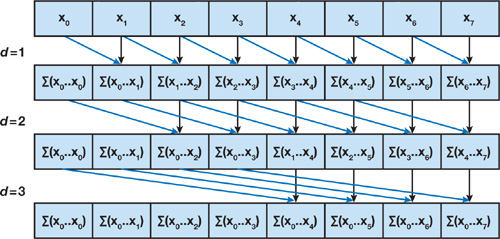
\includegraphics[width=0.5\linewidth]{scan_naive}
\caption{A naive approach for a parallel scan \cite{gpu_gems_3_chapter_39}.}
\label{fig:scan_naive}
\end{figure}

\lstset{basicstyle=\ttfamily{}\scriptsize{}}
\lstinputlisting[language=CL, caption=OpenCL Kernel code for the naive scan algorithm., label=lst:matrix_cl_naive_kernel]{../src/scan/gpu/thesis/NaiveScan.cl}
\lstset{basicstyle=\ttfamily{}}



extremely bad performance, why?

\subsection{Work efficient GPU implementation}

tree based approach (GPU Gems) work efficiency?

\begin{figure}
\centering
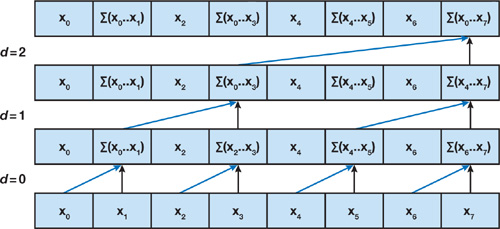
\includegraphics[width=0.5\linewidth]{scan_work_efficient_up_sweep}
\caption{The up-sweep phase of a work efficient parallel scan \cite{gpu_gems_3_chapter_39}.}
\label{fig:scan_work_efficient_up_sweep}
\end{figure}

\begin{figure}
\centering
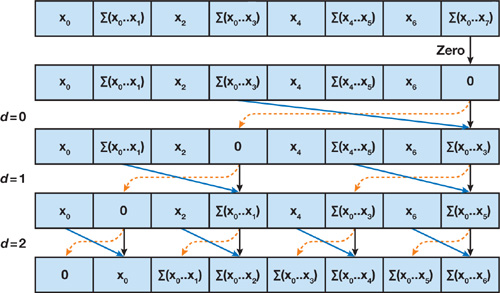
\includegraphics[width=0.5\linewidth]{scan_work_efficient_down_sweep}
\caption{The down-sweep phase of a work efficient parallel scan \cite{gpu_gems_3_chapter_39}.}
\label{fig:scan_work_efficient_down_sweep}
\end{figure}



maybe kernel code with explanation
runtime (diagram), memory transfer vs. calculation

\subsection{Existing implementations}
Apple
libCL
(AMD APP SDK Samples)
NVIDIA OpenCL Samples
common diagram

\subsection{Conclusion}
Why linear problems are still required on GPUs? (as building block for other algorithms)
commmon diagram
